\documentclass{article}
\usepackage{amsmath}
\usepackage{amsthm}
\usepackage{amsfonts}
\usepackage{mathtools}
\usepackage{listings}
\title{MATH 620: Homework 3}
\author{Fernando}
\date{October 17, 2023}
\begin{document}
\maketitle
\section{Problem 1}
\subsection{Part a}
In this case
\[
	f(x,u,\xi)=\mu(\sqrt{1+(u')^2}-1)-gu,
\]
so
\[ f_u=-g \]
\[ f_\xi =\frac{\mu u'}{\sqrt{1+(u')^2}} \]
\[ \frac{d}{dx} f_\xi =\frac{\mu u''}{(1+(u')^2)^{3/2}}. \]
Then the E-L equation is
\[
\frac{\mu u''}{(1+(u')^2)^{3/2}} = -g,
\]
or equivalently:
\[
\mu u'' -g\cdot(1+(u')^2)^{3/2} = 0,
\]
with initial conditions $u(a)=u(b)=1$.
\subsection{Part b}
In order to prove that $\overline u$ is a minimizer it is enough to show that
the map $(x,\xi)\mapsto f(x,u,\xi)$ is convex for every $x$.
In other words: is the function
\[
	h((x,y))=\mu(\sqrt{1+y^2} -1) -gx
\]
convex?

The answer is yes. We can see that this function is linear in $x$ and for $y$
we have that
\[
	\partial_{yy} h = \frac{\mu}{(1+y^2)^{3/2}}.
\]
In this particular case this is enough to conclude that the function is convex.
Because it is convex in the $y$ direction and linear in the $x$ direction. This
is an intuitive explanation, if we want to be more precise we can compute the
Hessian matrix but we will get the same result.

\textbf{Uniqueness?}

TODO
\section{Problem 2}
\subsection{Part a}
With this approcimation we have
\[
	f(x,u,u')=\frac{\mu}{2}(u')^2 -gu,
\]
so
\[
	f_u=-g
\]
\[
	f_\xi=\mu u'
\]
\[
	\frac{d}{dx}f_\xi = \mu u'',
\]
then
\[
	\mu u''=-g
\]
with same initial conditions, i.e. $u(a)=u(b)=1$.
\subsection{Part b}
For this part we can proceed exactly as before and we see that the map
$(u,\xi)\mapsto f(x,u,\xi)$ is convex for every $x$. So the solution is indeed
a minimizer.

\textbf{Uniqueness?}

TODO
\subsection{Part c}
By integrating the E-L equation two times we get that
\[
	u=-\frac{g}{2\mu} x^2 +c_1x+c_2.
\]
Using the conditions on the boundary we find $c_1$ and $c_2$. In this case
\[
	c_1=\frac{g}{2\mu}(a+b)
\]
and
\[
	c_2=1+\frac{g}{2\mu}a^2-c_1a.
\]
\section{Problem 3}
If we let $\lambda=\sqrt{\frac{1}{2g}}$ then
\[
	f(x,u,\xi)=\lambda(1+\xi^2)^{1/2}(H-u)^{-1/2}.
\]
Then
\[
	f_u=\frac{\lambda}{2}(1+\xi^2)^{1/2}(H-u)^{-3/2}
\]
and
\[
	f_\xi=\lambda\xi(1+\xi^2)^{-1/2}(H-u)^{-1/2}
\]
so the E-L equation becomes
\[
	\frac{d}{dx}(\lambda\xi(1+\xi^2)^{-1/2}(H-u)^{-1/2})
	=\frac{\lambda}{2}(1+\xi^2)^{1/2}(H-u)^{-3/2},
\]
with initial conditions $u(0)=H$ and $u(L)=0$.

Now we analyse the convexity of
\[
	h(x,y)=\lambda (1+y^2)^{1/2}(H-x)^{-1/2}.
\]
We can see that if we fix $x$ we get a strictly convex function and if we fix
$y$ again we get a strictly convex function. On top of that we see
that $h$ is smooth so intuitively it makes sense that this function
is strictly convex, if we want a rigorous argument we could take the Hessian
but this would be a lot of calculation. The figure below shows a plot of the
function which also suggests that the function is convex.

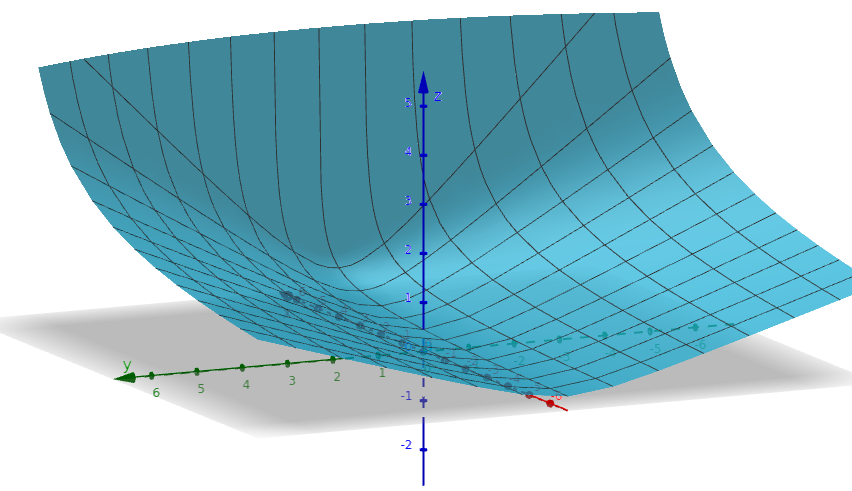
\includegraphics[width=0.9\textwidth]{convex.png}

This allows us to conjecture that the solution is unique.
\section{Problem 4}
Notation: $f_\xi = (f_{\xi_1},\dots,f_{\xi_n})$
Following the proof we saw in class we start with
\begin{align*}
	0=DI[u](v)
	&= \lim_{\varepsilon \to 0}\frac{I[u+\varepsilon v]-I[u]}{\varepsilon}\\
	&=\lim_{\varepsilon \to 0} \frac{1}{\varepsilon}\int_\Omega f(x,u+\varepsilon v,\nabla u+\varepsilon
	\nabla v)-f(x,u,\nabla u)\\
	&=\int_\Omega vf_u(x,u,\nabla u)+\nabla v\cdot f_\xi(x,u,\nabla u)\\
	&=\int_\Omega vf_u+\nabla v\cdot f_\xi.
\end{align*}
Using integration by parts (divergence theorem) we get:
\begin{align*}
	\int_\Omega\nabla v \cdot f_\xi
	&= \int_{\partial\Omega}v (f_\xi \cdot n) - \int_\Omega v (\nabla \cdot f_\xi)\\
	&= - \int_\Omega v (\nabla \cdot f_\xi),
\end{align*}
and observe that the boundary term is 0 because $v$ is 0 at
the boundary.
Then we get
\[
	0=\int_\Omega v(f_u-\nabla \cdot f_\varepsilon).
\]
Using the fundamental theorem of calculus in variations we get the E-L
equation
\[
	f_u=\nabla \cdot f_\varepsilon.
\]
\section{Problem 5}
% LEAL
\end{document}
